\chapter{Лабораторная работа №5. Создание IP ядра с управлением по AXI4-Lite}

\section{Интерфейс AXI4-Lite}

Интерфейс AXI4-Lite состоит из следующих независимых каналов транзакций:

\begin{itemize}
	\item Read Address Channel, кратко AR
	\item Write Address Channel, кратко AW
	\item Read Data Channel, кратко R
	\item Write Data Channel, кратко W  
	\item Write Response Channel, кратко B
\end{itemize}

На рисунках~\ref{AXI_read_channel} и~\ref{AXI_write_ch} представлена архитектура каналов AXI4-Lite, а в таблицах ~\ref{WA} - ~\ref{WRC} представлено описание всех пяти каналов интерфейса AXI4.

Read Address Channel предназначен для передачи управляющей информации и адреса чтения от ведущего(master) к ведомому(slave) для совершения транзакции чтения. Read Data Channel предназначен для передачи данных от ведомого к ведущему. Транзакция чтения происходит следующим образом: ведущий передаёт управляющую информацию и адрес чтения ведомому на канале AR, если тот принял её, то он формирует ответ на канале R c запрошенными данными.

Write Address Channel предназначен для передачи управляющей информации от ведущего к ведомому для совершения транзакции записи.Write Data Channel предназначен для передачи данных от ведущего к ведомому при записи данных. Write Response Channel предназначен для формирования ответа ведомым о состоянии транзакции записи. Транзакция записи происходит следующим образом: ведущий передаёт управляющую информацию и адрес записи ведомому на канале AW, если тот принял её, то на канале W ведущий формирует транзакцию записи, после этого ожидаем ответ на канале B. 

\begin{figure}[htbp]	
	\subfigure[Архитектура канала чтения интерфейса AXI] 
	{
		\begin{minipage}{8cm}
			\centering         
			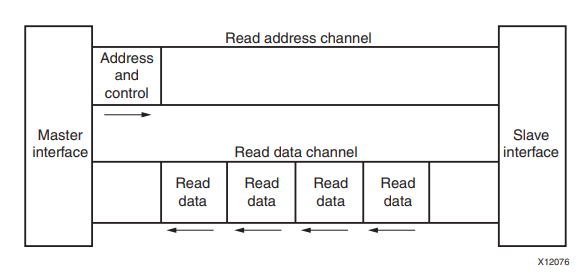
\includegraphics[scale=0.4]{image/AXI_read_ch.png}   
			\label{AXI_read_channel}
		\end{minipage}
	}
	\subfigure[Архитектура канала записи интерфейса AXI] 
	{
		\begin{minipage}{8cm}
			\centering      
			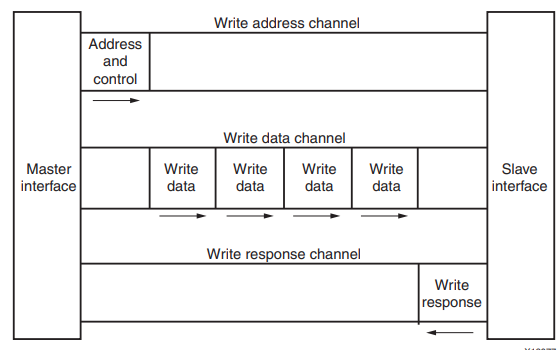
\includegraphics[scale=0.4]{image/AXI_write_ch.png}   
			\label{AXI_write_ch}
		\end{minipage}
	}
	\caption{Архитектура каналов чтения и записи в AXI} %  %Имя большого изображения
\end{figure}

\renewcommand{\arraystretch}{1.1} %% increase table row spacing

\begin{table}[!ht]
	\centering
	\caption{Cигналы Write Address Channel AXI4-Lite}
	\label{WA}
	\begin{tabular}{c c p{0.6\textwidth}} 
		\toprule
		Сигнал & Источник & Описание \\ 
		\midrule
		AWADDR & Master & Адрес записи. Адрес записи дает адрес 
		первой передачи при пакетной транзакции. \\
		AWVALID & Master  & \multirow{2}{*}{Сигналы механизма "рукопожатий".} \\ 
		AWREADY & Slave  &   \\
		\bottomrule
	\end{tabular}
\end{table}

\begin{table}[!ht]
		\centering
		\caption{Описание сигналов Read Address Channel интерфейса AXI4-Lite}
		\label{RA}
		\begin{tabular}{ c  c  p{0.6\textwidth} } 
			\toprule
			Сигнал & Источник & Описание \\ 
			\midrule 
			ARADDR & Master & Адрес по которому будет происходит операция чтения данных. Для пакетной транзакции дает адрес первой операции чтения.\\
			ARVALID & Master  & \multirow{2}{*}{Сигналы механизма "рукопожатий".} \\ 
			ARREADY & Slave  & \\
			\bottomrule
		\end{tabular}
\end{table}

\begin{table}[!ht]
	\centering
	\caption{Сигналы Write Data Channel AXI4-Lite}
	\label{WD}
	\begin{tabular}{ c  c  p{0.6\textwidth} } 
		\toprule
		Сигнал & Источник & Описание \\ 
		\midrule
		WDATA & Master & Шина данных записи. \\ 
		WSTRB & Master  & Cтробы данных записи. Этот сигнал указывает, какие байты содержат действительные данные. На каждые восемь бит шины данных записи приходится один стробирующий бит записи. \\ 
		WVALID & Slave  & \multirow{2}{*}{Сигналы механизма "рукопожатий".} \\ 
		WREADY & Slave  & \\
		\bottomrule
	\end{tabular}

\end{table}

\begin{table}[!ht]
	\centering
	\caption{Сигналы Read Data Channel AXI4-Lite}
	\label{RD}
		\begin{tabular}{  c c  p{0.6\textwidth} } 
			\toprule
			Сигнал & Источник & Описание \\ 
			\midrule
			RDATA & Slave & Прочитанные данные. \\ 
			RRESP & Slave  & Этот сигнал указывает на состояние транзакции чтения. \\ 
			RVALID & Slave  & \multirow{2}{*}{Сигналы механизма "рукопожатий".} \\ 
			RREADY & Master  & \\ 
			\bottomrule
		\end{tabular}
\end{table}

\begin{table}[!ht]
	\centering
	\caption{Сигналы Write Response Channel AXI4-Lite}
	\label{WRC}
		\begin{tabular}{  c c  p{0.6\textwidth} } 
			\toprule
			Сигнал & Источник & Описание \\
			\midrule
			BRESP & Slave  & Ответ на запись. Этот сигнал указывает на состояние транзакции записи. \\
			BVALID & Slave  & \multirow{2}{*}{Сигналы механизма "рукопожатий".} \\ 
			BREADY & Master  & \\ 
			\bottomrule
		\end{tabular}
\end{table}

\clearpage

Рассмотрим механизм обмена данными в AXI4. Все пять каналов транзакций используют один и тот же процесс подтверждения VALID/READY для передачи адреса, данных и управляющей информации. Этот двусторонний механизм управления потоком означает, что и ведущий, и ведомый могут управлять скоростью, с которой информация перемещается между ведущим и ведомым. Источник генерирует сигнал VALID, чтобы указать, когда адрес, данные или управляющая информация доступны. Приёмник генерирует сигнал READY, чтобы указать, что он может принять информацию. Передача происходит только тогда, когда оба сигнала VALID и READY имеют высокий уровень.

\begin{figure}[!ht]
	\centering
	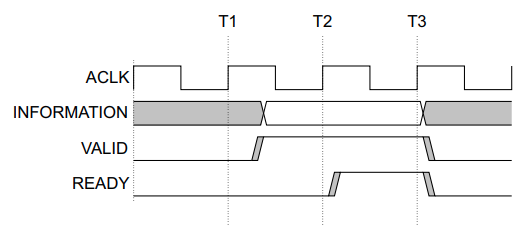
\includegraphics[width=0.4\textwidth]{image/AXI-handshape}
	\caption{Механизм обмена данными - VALID до READY}
	\label{AXI-valid_before_ready}
\end{figure}

На рисунке~\ref{AXI-valid_before_ready} источник представляет адрес, данные или управляющую информацию после T1 и утверждает сигнал VALID. Приёмник устанавливает сигнал READY после T2, а источник должен сохранять свою информацию стабильной до тех пор, пока передача не произойдет в T3.


\begin{figure}[!ht]
	\centering
	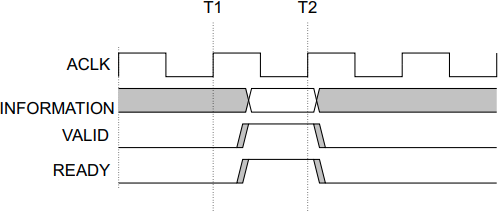
\includegraphics[width=0.4\textwidth]{image/AXI-hand-valid}
	\caption{Механизм обмена данными - READY и VALID одновременно}
	\label{AXI-valid_ready}
\end{figure}


На рисунке~\ref{AXI-valid_ready} и источник, и приёмник после T1 указывают, что они могут передавать/принимать адрес, данные или управляющую информацию. В этом случае передача происходит по нарастающему фронту тактового сигнала T2, когда как VALID, так и READY имеют высокий уровень напряжения.

\begin{figure}[!ht]
	\centering
	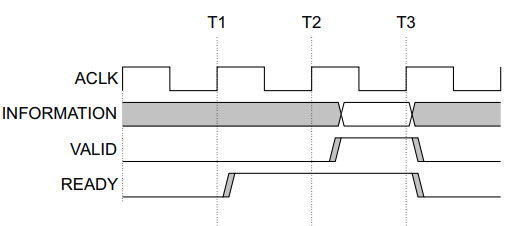
\includegraphics[width=0.4\textwidth]{image/AXI-hand_ready}
	\caption{Механизм обмена данными - READY до VALID}
	\label{AXI-handshape}
\end{figure}

На рисунке~\ref{AXI-handshape} приёмник утверждает READY после T1, прежде чем адрес, данные или управляющая информация являются действительными, указывая на то, что он может принять информацию. Источник представляет информацию и утверждает VALID после T2, и передача происходит в T3.

\section{Транзакции чтения и записи интерфейса AXI4-Lite}

На рисунке ~\ref{AXI_wr_tr} представлен пример транзакции записи интерфейса AXI4-Lite.
Опишем последовательность выполнения транзакции.

\begin{figure}[h]
	\centering
	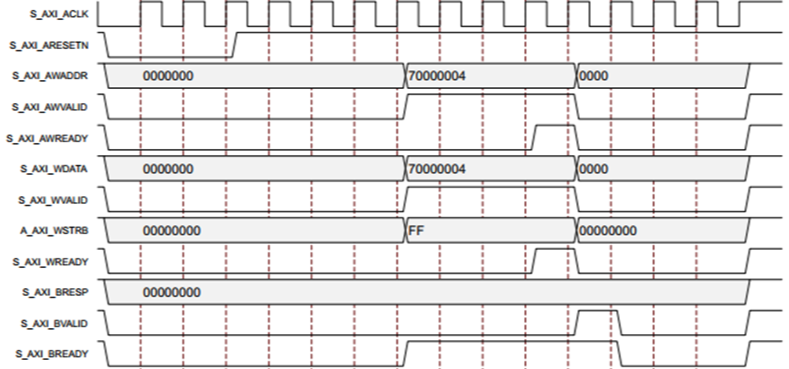
\includegraphics[width=0.8\textwidth]{image/axi_lite_write}
	\caption{AXI4-Lite транзакция записи}
	\label{AXI_wr_tr}
\end{figure}

\begin{enumerate}
	\item Мастер помещает адрес в канал адреса записи, а данные - в канал данных записи. В то же время он утверждает AWVALID и WVALID, указывая, что адрес и данные на соответствующих каналах действительны. BREADY также утверждается Мастером, указывая на то, что он готов получить ответ.
	\item Подчиненное устройство устанавливает AWREADY и WREADY на каналы адреса записи и записи данных соответственно.
	\item Поскольку сигналы «Действительный» и «Готово» присутствуют как на каналах адреса записи, так и на каналах записи данных, на этих каналах происходит подтверждение связи, и соответствующие сигналы «Действительный» и «Готово» могут быть отменены. (После того, как произойдут оба рукопожатия, ведомое устройство имеет адрес записи и данные)
	\item Подчиненное устройство заявляет BVALID, указывая на наличие действительного ответа по каналу ответа на запись. (в данном случае ответ 2'b00, это «ОК»).
	\item Следующий нарастающий фронт тактовой частоты завершает транзакцию, при этом сигналы Ready и Valid в канале ответа на запись имеют высокий уровень.
\end{enumerate}

На рисунке ~\ref{AXI_wr_tr} представлен пример транзакции чтения интерфейса AXI4-Lite.
Опишем последовательность выполнения транзакции.

\begin{figure}[h]
	\centering
	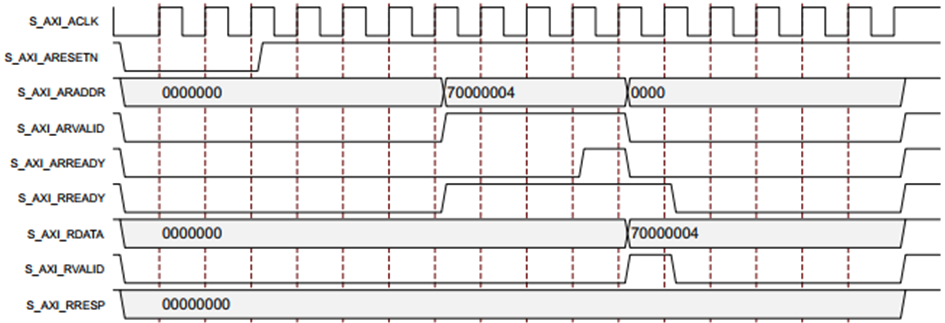
\includegraphics[width=0.8\textwidth]{image/axi_lite_read}
	\caption{AXI4-Lite транзакция чтения}
	\label{AXI_rd_tr}
\end{figure}

\begin{enumerate}
	\item Мастер помещает адрес в канал адреса чтения, а также устанавливает ARVALID, указывая, что адрес действителен, и RREADY, указывая, что мастер готов принять данные от подчиненного устройства.
	\item Подчиненный заявляет ARREADY, указывая, что он готов принять адрес на шине.
	\item Поскольку подтверждены как ARVALID, так и ARREADY, на следующем нарастающем фронте тактового сигнала происходит квитирование, после чего ведущее и ведомое устройства отменяют ARVALID и ARREADY, соответственно. (На этом этапе ведомое устройство получило запрошенный адрес).
	\item Подчиненное устройство помещает запрошенные данные в канал чтения данных и устанавливает RVALID, указывая, что данные в канале действительны. Подчиненное устройство также может отправить ответ на RRESP, хотя здесь этого не происходит.
	\item Поскольку подтверждены и RREADY, и RVALID, следующий нарастающий фронт тактовой частоты завершает транзакцию. RREADY и RVALID теперь можно отключить.
\end{enumerate}

Подтверждения связи в канале адреса записи и записи данных не обязательно происходят одновременно (как в показанной транзакции). Однако спецификация AXI4 утверждает, что оба должны произойти, прежде чем ведомое устройство сможет отправить ответ на запись. Подтверждение адреса записи и записи данных может происходить независимо или одновременно, и никакой порядок не применяется, только оба должны произойти для завершения транзакции.

\section{AXI4-Lite и конфигурационные регистры ядра}

У ядра предусмотрен(если нужно) набор конфигурационных регистров. Чаще всего регистры сгруппированы по словам (например, 32-битным), где внутри разделяются по полям(в пределах одного регистра могут быть несколько полей), у которых могут быть различные режимы работы:
\begin{enumerate}
	\item RW — read and write: можно писать и читать. Служат для настройки ядра (например, включение того или иного режима работы, настройка каких-то параметров и пр.).
	\item RW/SC — read write self clear: если записать единицу, то она сама сбросит в ноль (может быть удобно для ресета ядра или модуля ядра: ставишь единицу, а он сам сбросит себя в ноль).
	\item RO — read only: только читать (например, для статистики или о состояния ядра). Так же некоторые регистры делаются RO для хранения константных значений (например, версию ядра, либо его возможности).
\end{enumerate}

Конфигурационные регистры так же есть у различных микросхем, таких как аналого-цифровые и цифро-аналоговые преобразователи, системы фазовой автоподстройки частоты, микросхемы реализующие физический уровень интерфейса Ethernet и у многих других.

При проектирование цифровых устройств на ПЛИС фирмы Xilinx конфигурационные регистры ядра чаще всего реализуются с использованием интерфейса AXI4-Lite. Среда разработки Vivado Design Suite при создании проекта IP ядра позволяет получить код ведомого(slave) интерфейса AXI4-Lite, который можно легко использовать для создания системы конфигурационных регистров ядра. Укажем, что кроме этого генерировать можно ведущий(master) интерфейс AXI4-Lite, а также ведущий(master) и ведомый(slave) таких интерфейсов как AXI4 и AXI4-Stream.

\section{Создание IP ядра в Vivado}

Для создания собственного IP ядра в Vivado нажмите \verb|Tools -> Create and Package New Ip...|(см. рис. ~\ref{create_and_pkg_new_ip_0}, ~\ref{create_and_pkg_new_ip_1}).
Во вкладке \verb|Create Peripheral, Package IP or Package a Block Deisgn| выбираем пункт создания ядра с AXI4 интерфейсом: \verb|Create a new AXI4 peripheral|(см. рис. ~\ref{create_and_pkg_new_ip_2}). В следующей вкладке \verb|Peripheral Details| введите имя, версию, описание и путь до ядра как показано на~\ref{create_and_pkg_new_ip_3}.

\begin{figure}[htbp]	
	\subfigure[Tools->Create and Package New Ip...] 
	{
		\begin{minipage}{8cm}
			\centering         
			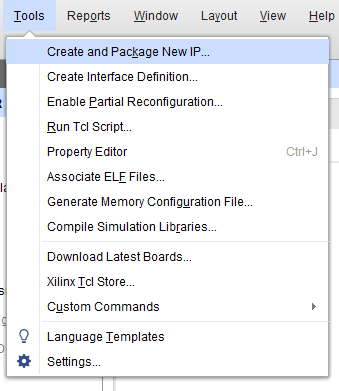
\includegraphics[scale=0.5]{image/create_and_pkg_new_ip_0.png}   
			\label{create_and_pkg_new_ip_0}
		\end{minipage}
	}
	\subfigure[Окно мастера создания IP ядра] 
	{
		\begin{minipage}{8cm}
			\centering      
			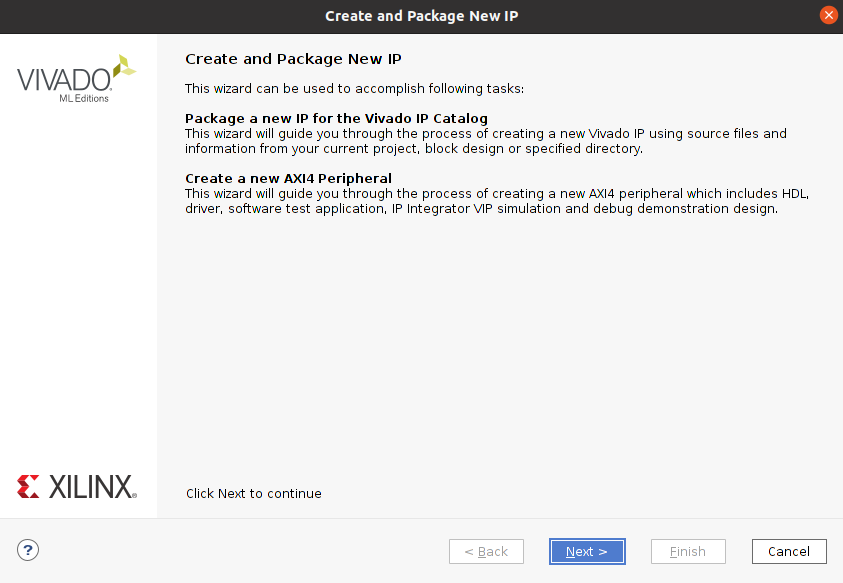
\includegraphics[scale=0.3]{image/create_and_pkg_new_ip_1.png}   
			\label{create_and_pkg_new_ip_1}
		\end{minipage}
	}
	\caption{Запуск мастера создания IP ядра} %  %Имя большого изображения
\end{figure}


\begin{figure}[htbp]	
	\subfigure[Create a new AXI4 peripheral] 
	{
		\begin{minipage}{8cm}
			\centering         
			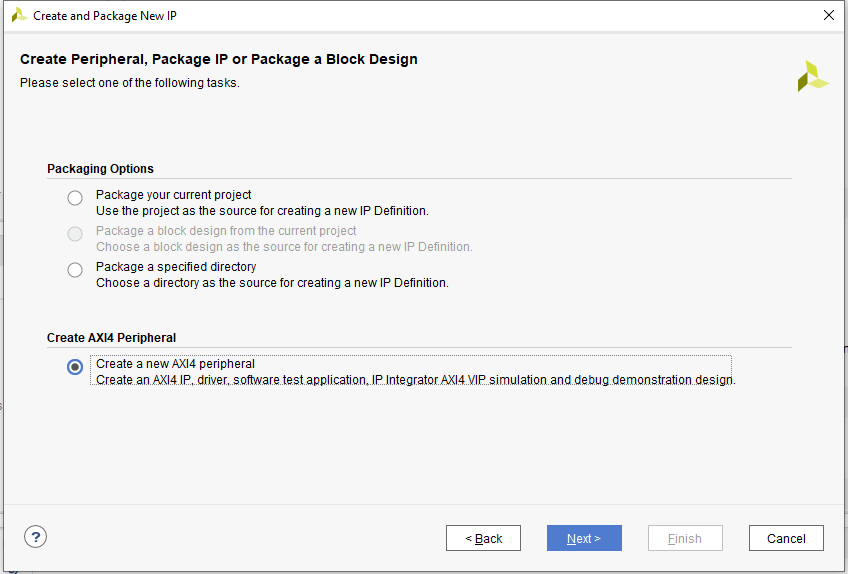
\includegraphics[scale=0.3]{image/create_and_pkg_new_ip_2.png}   
			\label{create_and_pkg_new_ip_2}
		\end{minipage}
	}
	\subfigure[Создаём параметры нового IP ядра] 
	{
		\begin{minipage}{8cm}
			\centering      
			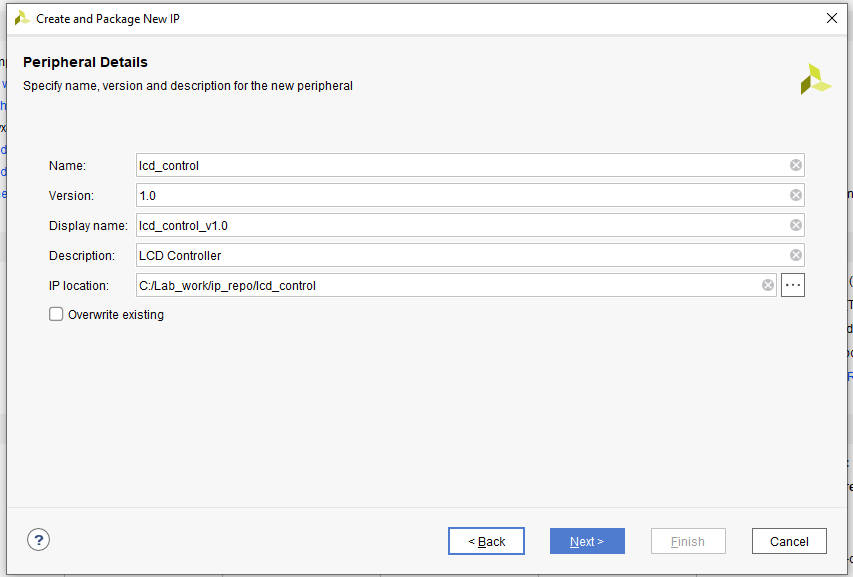
\includegraphics[scale=0.3]{image/create_and_pkg_new_ip_3.png}   
			\label{create_and_pkg_new_ip_3}
		\end{minipage}
	}
	\caption{Тип и параметры ядра} %  %Имя большого изображения
\end{figure}

\begin{figure}[htbp]	
	\subfigure[Выбор интерфейса] 
	{
		\begin{minipage}{8cm}
			\centering         
			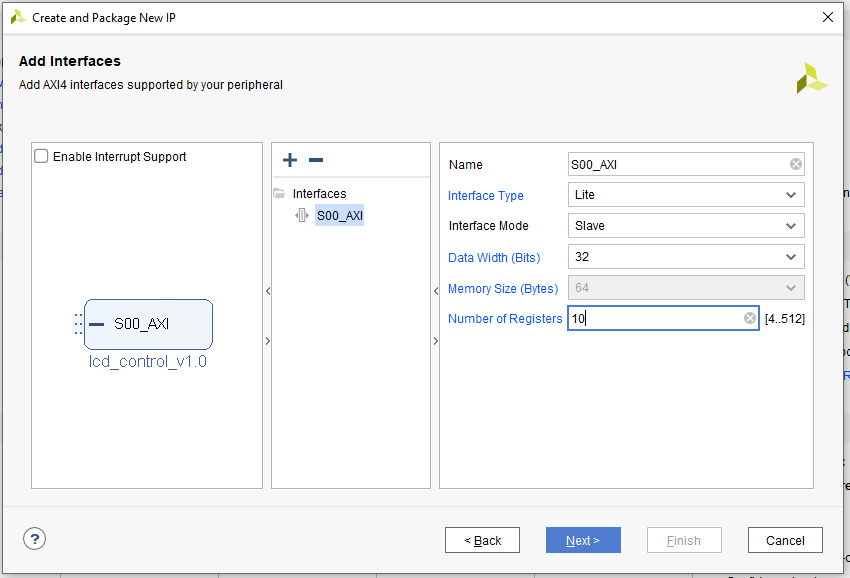
\includegraphics[scale=0.3]{image/create_and_pkg_new_ip_4.png}   
			\label{create_and_pkg_new_ip_4}
		\end{minipage}
	}
	\subfigure[Выбор следующий шага после генерации ядра] 
	{
		\begin{minipage}{8cm}
			\centering      
			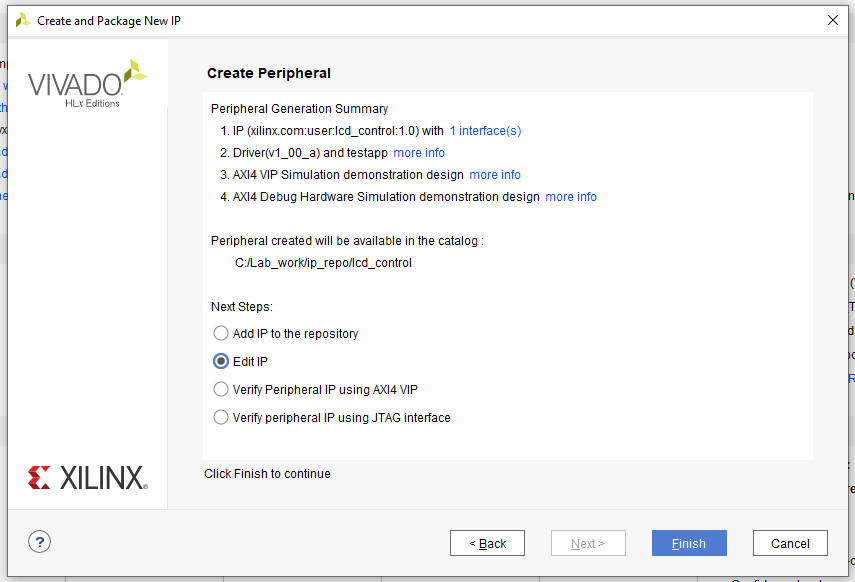
\includegraphics[scale=0.3]{image/create_and_pkg_new_ip_5.png}   
			\label{create_and_pkg_new_ip_5}
		\end{minipage}
	}
	\caption{Выбор интерфейса и следующего шага после генерации ядра} %  %Имя большого изображения
\end{figure}

\begin{Verbatim}[tabsize=4]
module lcd #(
	parameter CYCLES_PER_US = 50
)
(
	input wire clk,    
	input wire rst, 
	output wire [2:0] ctrl_lcd,
	output wire [3:0] data_lcd,

	output wire 		lcd_ready,
 	input wire 			lcd_valid,
 	input wire [31:0] 	lcd_data_str_0_0,
 	input wire [31:0] 	lcd_data_str_0_1,
 	input wire [31:0] 	lcd_data_str_0_2,
 	input wire [31:0] 	lcd_data_str_0_3,
 	input wire [31:0] 	lcd_data_str_1_0,
 	input wire [31:0] 	lcd_data_str_1_1,
 	input wire [31:0] 	lcd_data_str_1_2,
 	input wire [31:0] 	lcd_data_str_1_3
);

	localparam [3:0]
		WAITING = 4'd0,
        INIT_H30_ONE = 4'd1,
        INIT_H30_TWO = 4'd2,
        INIT_H30_THREE = 4'd3,
        INIT_H20 = 4'd4,
        INIT_FUNCTION_SET = 4'd5,
        INIT_DISPLAY_ON = 4'd6,
		INIT_DISPLAY_CLEAR = 4'd7,
		INIT_SET_ENTRY_MODE = 4'd8,
		CUR_FIRST_ROW = 4'd9,
		WRITE_UPPER_LINE = 4'd10,
		COUNTER_UPPER_LINE = 4'd11,
		CUR_SECOND_ROW = 4'd12,
		WRITE_LOWER_LINE = 4'd13,
		COUNTER_LOWER_LINE = 4'd14,
		LCD_WAIT_VALID = 4'd15;

	reg lcd_ready_r;

	assign lcd_ready = lcd_ready_r;

\end{Verbatim}

\begin{Verbatim}[tabsize=4]
               	LCD_WAIT_VALID: begin
               		if(lcd_valid) begin
               			lcd_ready_r <= 1'b0;
               			lcd_state_r <= CUR_FIRST_ROW;
               			upper_line[0] <= lcd_data_str_0_0[7:0]; 
						upper_line[1] <= lcd_data_str_0_0[15:8]; 
						upper_line[2] <= lcd_data_str_0_0[23:16];
						upper_line[3] <= lcd_data_str_0_0[31:24];
						upper_line[4] <= lcd_data_str_0_1[7:0]; 
						upper_line[5] <= lcd_data_str_0_1[15:8]; 
						upper_line[6] <= lcd_data_str_0_1[23:16]; 
						upper_line[7] <= lcd_data_str_0_1[31:24]; 
						upper_line[8] <=  lcd_data_str_0_2[7:0];  
						upper_line[9] <=  lcd_data_str_0_2[15:8]; 
						upper_line[10] <= lcd_data_str_0_2[23:16]; 
						upper_line[11] <= lcd_data_str_0_2[31:24]; 
						upper_line[12] <= lcd_data_str_0_3[7:0]; 
						upper_line[13] <= lcd_data_str_0_3[15:8]; 
						upper_line[14] <= lcd_data_str_0_3[23:16]; 
						upper_line[15] <= lcd_data_str_0_3[31:24]; 

               			lower_line[0] <= lcd_data_str_1_0[7:0]; 
						lower_line[1] <= lcd_data_str_1_0[15:8];
						lower_line[2] <= lcd_data_str_1_0[23:16]; 
						lower_line[3] <= lcd_data_str_1_0[31:24]; 
						lower_line[4] <= lcd_data_str_1_1[7:0]; 
						lower_line[5] <= lcd_data_str_1_1[15:8];
						lower_line[6] <= lcd_data_str_1_1[23:16]; 
						lower_line[7] <= lcd_data_str_1_1[31:24];
						lower_line[8] <=  lcd_data_str_1_2[7:0];
						lower_line[9] <=  lcd_data_str_1_2[15:8]; 
						lower_line[10] <= lcd_data_str_1_2[23:16];
						lower_line[11] <= lcd_data_str_1_2[31:24];
						lower_line[12] <= lcd_data_str_1_3[7:0]; 
						lower_line[13] <= lcd_data_str_1_3[15:8]; 
						lower_line[14] <= lcd_data_str_1_3[23:16]; 
						lower_line[15] <= lcd_data_str_1_3[31:24]; 
               		end else begin
               			lcd_ready_r <= 1'b1;
						lcd_state_r <= LCD_WAIT_VALID;
               		end
               	end
\end{Verbatim}

\begin{Verbatim}[tabsize=4]
				COUNTER_LOWER_LINE: begin
               		if(counter_lower_line_r == 32'd15) begin
						counter_lower_line_r <= 32'b0;
						lcd_state_r <= LCD_WAIT_VALID;		
                	end else begin
	                	counter_lower_line_r <= counter_lower_line_r + 1;
	                	lcd_state_r <= WRITE_LOWER_LINE;
                	end
               	end
\end{Verbatim}
\section{Верификация ядра с интерфейсом AXI4-Lite}
Если мы разрабатываем ядро, реализуя конфигурационные регистры с использованием ведомого интерфейса AXI4-Lite, то при тестировании ядра необходимо в соответствии с логикой работы ядра заполнить конфигурационные регистры. Для этого необходимо написать тестбенч для ведущего(мастера) интерфейса AXI4-Lite.

\begin{Verbatim}[tabsize=4]
`timescale 1ns/1ps

module tb_lcd();
	
	parameter integer AXI_DATA_WIDTH = 32;
	parameter integer AXI_ADDR_WIDTH = 6;
	parameter integer T_SYS_CLK = 5;


	parameter integer ADDR_DATA_STR_0_0 = 0;
	parameter integer ADDR_DATA_STR_0_1 = 4;
	parameter integer ADDR_DATA_STR_0_2 = 8;
	parameter integer ADDR_DATA_STR_0_3 = 12;
	parameter integer ADDR_DATA_STR_1_0 = 16;
	parameter integer ADDR_DATA_STR_1_1 = 20;
	parameter integer ADDR_DATA_STR_1_2 = 24;
	parameter integer ADDR_DATA_STR_1_3 = 28;
	parameter integer ADDR_VALID 		= 36;


	reg [AXI_ADDR_WIDTH - 1:0] 	axil_awaddr;
	reg 						axil_awvalid;
	wire 						axil_awready;
	
	reg [AXI_DATA_WIDTH - 1:0] 	axil_wdata;
	wire 						axil_wready;
	reg 	 					axil_wvalid;
	
	reg 	 					axil_bready;
	wire 						axil_bvalid;

	reg [AXI_ADDR_WIDTH - 1:0] 	axil_araddr;
	reg 						axil_arvalid;
	wire 						axil_arready;
	
	wire [AXI_DATA_WIDTH - 1:0] axil_rdata;
	reg 						axil_rready;
	wire 						axil_rvalid;

	reg [7:0] upper_line [15:0];
	reg [7:0] lower_line [15:0];

	reg sys_clk;
	reg sys_rst;

	initial 
		sys_clk = 1'b0;
	always 
		sys_clk = #(T_SYS_CLK/2) ~sys_clk;

	task delayT_t;
		input [31:0] T;
		input [31:0] N;
		begin
			repeat (N)
			#T;
		end
	endtask
	
	task AXI4_Lite_W;
		input [31:0] T;
		input [31:0] ADDR;
		input [31:0] DATA;
		begin
			delayT_t(T,2);
			axil_awaddr <= ADDR;
			axil_awvalid <= 1;
			axil_wdata <= DATA;
			axil_wvalid <= 1;
			axil_bready <= 0;
			wait (axil_awready || axil_wready);
			if (axil_awready && axil_wready) begin
				delayT_t(T,1);
				axil_awvalid <= 0;
				axil_wvalid <= 0;
			end else if (axil_awready) begin
				delayT_t(T,1);
				axil_awvalid <= 0;
				wait(axil_wready);
				delayT_t(T,1);
				axil_wvalid <= 0;
			end else if (axil_wready) begin
				delayT_t(T,1);
				axil_wvalid <= 0;
				wait(axil_awready);
				delayT_t(T,1);
				axil_awvalid <= 0;
			end
			axil_bready <= 1;
			wait(axil_bvalid);
			delayT_t(T,1);
			axil_bready <= 0;
		end
	endtask

	task AXI4_Lite_R;
		input [31:0] T;
		input [31:0] ADDR;
		output [31:0] DATA;
		begin
			delayT_t(T,2);
			axil_araddr <= ADDR;
			axil_arvalid <= 1;
			wait(axil_arready);
			delayT_t(T,1);
			axil_arvalid <= 0;
			axil_rready <= 1;
			wait(axil_rvalid);
			delayT_t(T,1);
			DATA <= axil_rdata;
			axil_rready <= 0;
		end
	endtask

	initial begin
		upper_line[0] = 8'h46; // F
		upper_line[1] = 8'h69; // i
		upper_line[2] = 8'h72; // r
		upper_line[3] = 8'h6d; // m
		upper_line[4] = 8'h77; // w
		upper_line[5] = 8'h61; // a
		upper_line[6] = 8'h72; // r
		upper_line[7] = 8'h65; // e
		upper_line[8] = 8'h20; // 
		upper_line[9] = 8'h6c; // l
		upper_line[10] = 8'h6f; // o
		upper_line[11] = 8'h61; // a
		upper_line[12] = 8'h64; // d
		upper_line[13] = 8'h65; // e
		upper_line[14] = 8'h64; // d
		upper_line[15] = 8'h21; // !
				
		lower_line[0] = 8'h30; // 0
		lower_line[1] = 8'h31; // 1
		lower_line[2] = 8'h32; // 2
		lower_line[3] = 8'h33; // 3
		lower_line[4] = 8'h34; // 4
		lower_line[5] = 8'h35; // 5
		lower_line[6] = 8'h36; // 6
		lower_line[7] = 8'h37; // 7
		lower_line[8] = 8'h38; // 8
		lower_line[9] = 8'h39; // 9
		lower_line[10] = 8'h61; // a
		lower_line[11] = 8'h62; // b
		lower_line[12] = 8'h63; // c
		lower_line[13] = 8'h64; // d
		lower_line[14] = 8'h65; // e
		lower_line[15] = 8'h66; // f
	end

	initial begin
		axil_awaddr = 32'b0;
		axil_awvalid = 32'b0;
		axil_wdata = 32'b0;
		axil_wvalid = 32'b0;
		axil_bready = 32'b0;
		sys_rst = 1'b1;
	    delayT_t(5, 4000);
	    sys_rst = 1'b0;
		delayT_t(5, 10000000);

	    AXI4_Lite_W(T_SYS_CLK, ADDR_DATA_STR_0_0, {upper_line[0], upper_line[1], upper_line[2], upper_line[3]});
	    AXI4_Lite_W(T_SYS_CLK, ADDR_DATA_STR_0_1, {upper_line[4], upper_line[5], upper_line[6], upper_line[7]});
	    AXI4_Lite_W(T_SYS_CLK, ADDR_DATA_STR_0_2, {upper_line[8], upper_line[9], upper_line[10], upper_line[11]});
	    AXI4_Lite_W(T_SYS_CLK, ADDR_DATA_STR_0_3, {upper_line[12], upper_line[13], 	upper_line[14], upper_line[15]});

	    AXI4_Lite_W(T_SYS_CLK, ADDR_DATA_STR_1_0, {lower_line[0], lower_line[1], lower_line[2], lower_line[3]});
	    AXI4_Lite_W(T_SYS_CLK, ADDR_DATA_STR_1_1, {lower_line[4], lower_line[5], lower_line[6], lower_line[7]});
	    AXI4_Lite_W(T_SYS_CLK, ADDR_DATA_STR_1_2, {lower_line[8], lower_line[9], lower_line[10], lower_line[11]});
	    AXI4_Lite_W(T_SYS_CLK, ADDR_DATA_STR_1_3, {lower_line[12], lower_line[13], lower_line[14], lower_line[15]});

	    AXI4_Lite_W(T_SYS_CLK, ADDR_VALID, 32'h1);
	end

	top_lcd
	top_lcd_inst
	(
		.s00_axi_aclk(sys_clk),
		.s00_axi_aresetn(~sys_rst),

		.s00_axi_awaddr(axil_awaddr),
		.s00_axi_awprot(3'b0),
		.s00_axi_awvalid(axil_awvalid),
		.s00_axi_awready(axil_awready),

		.s00_axi_wdata(axil_wdata),
		.s00_axi_wstrb(4'b1111),
		.s00_axi_wvalid(axil_wvalid),
		.s00_axi_wready(axil_wready),

		.s00_axi_bresp(),
		.s00_axi_bvalid(axil_bvalid),
		.s00_axi_bready(axil_bready),

		.s00_axi_araddr(),
		.s00_axi_arprot(),
		.s00_axi_arvalid(),
		.s00_axi_arready(),

		.s00_axi_rdata(),
		.s00_axi_rresp(),
		.s00_axi_rvalid(),
		.s00_axi_rready(),

		.lcd_data(), 
		// LCD: E   (control bit)	
		.lcd_e(),	
		// LCD: RS  (setup or data)
		.lcd_rs(),	
		// LCD: R/W (read or write)
		.lcd_rw()	
	);

endmodule
\end{Verbatim}

\section{Проект в Vivado}

\section{Проект в Xilinx SDK}

\begin{Verbatim}[tabsize=4]
#include <stdio.h>
#include "platform.h"
#include "xil_printf.h"
#include "xgpio.h"
#include "xparameters.h"
#include "sleep.h"
#include "string.h"

XGpio gpio;

#define MYIP_S00_AXI_SLV_REG0_OFFSET 0
#define MYIP_S00_AXI_SLV_REG1_OFFSET 4
#define MYIP_S00_AXI_SLV_REG2_OFFSET 8
#define MYIP_S00_AXI_SLV_REG3_OFFSET 12
#define MYIP_S00_AXI_SLV_REG4_OFFSET 16
#define MYIP_S00_AXI_SLV_REG5_OFFSET 20
#define MYIP_S00_AXI_SLV_REG6_OFFSET 24
#define MYIP_S00_AXI_SLV_REG7_OFFSET 28
#define MYIP_S00_AXI_SLV_REG8_OFFSET 32
#define MYIP_S00_AXI_SLV_REG9_OFFSET 36

int main()
{
	init_platform();

	xil_printf("Hello World\n\r");
	u32 i = 0;
	u32 led = 0;

	XGpio_Initialize(&gpio, XPAR_GPIO_0_DEVICE_ID);

	char str_upper[16];
	char str_lower[16];

	strcpy(str_upper, "Microblaze Work!");
	strcpy(str_lower, "Firmware loaded!");

	u32 reg_0 = (str_upper[3] << 24) | (str_upper[2] << 16) | (str_upper[1] << 8) | str_upper[0];
	u32 reg_1 = (str_upper[7] << 24) | (str_upper[6] << 16) | (str_upper[5] << 8) | str_upper[4];
	u32 reg_2 = (str_upper[11] << 24) | (str_upper[10] << 16) | (str_upper[9] << 8) | str_upper[8];
	u32 reg_3 = (str_upper[15] << 24) | (str_upper[14] << 16) | (str_upper[13] << 8) | str_upper[12];
	u32 reg_4 = (str_lower[3] << 24) | (str_lower[2] << 16) | (str_lower[1] << 8) | str_lower[0];
	u32 reg_5 = (str_lower[7] << 24) | (str_lower[6] << 16) | (str_lower[5] << 8) | str_lower[4];
	u32 reg_6 = (str_lower[11] << 24) | (str_lower[10] << 16) | (str_lower[9] << 8) | str_lower[8];
	u32 reg_7 = (str_lower[15] << 24) | (str_lower[14] << 16) | (str_lower[13] << 8) | str_lower[12];

	sleep(1);
	Xil_Out32(XPAR_MYIP_0_S00_AXI_BASEADDR + MYIP_S00_AXI_SLV_REG0_OFFSET, reg_0);
	Xil_Out32(XPAR_MYIP_0_S00_AXI_BASEADDR + MYIP_S00_AXI_SLV_REG1_OFFSET, reg_1);
	Xil_Out32(XPAR_MYIP_0_S00_AXI_BASEADDR + MYIP_S00_AXI_SLV_REG2_OFFSET, reg_2);
	Xil_Out32(XPAR_MYIP_0_S00_AXI_BASEADDR + MYIP_S00_AXI_SLV_REG3_OFFSET, reg_3);
	Xil_Out32(XPAR_MYIP_0_S00_AXI_BASEADDR + MYIP_S00_AXI_SLV_REG4_OFFSET, reg_4);
	Xil_Out32(XPAR_MYIP_0_S00_AXI_BASEADDR + MYIP_S00_AXI_SLV_REG5_OFFSET, reg_5);
	Xil_Out32(XPAR_MYIP_0_S00_AXI_BASEADDR + MYIP_S00_AXI_SLV_REG6_OFFSET, reg_6);
	Xil_Out32(XPAR_MYIP_0_S00_AXI_BASEADDR + MYIP_S00_AXI_SLV_REG7_OFFSET, reg_7);

	Xil_Out32(XPAR_MYIP_0_S00_AXI_BASEADDR + MYIP_S00_AXI_SLV_REG9_OFFSET, 0x1);

	while(1)
	{
		i++;
		if(i == 1000000)
		{
			led = !led;
			XGpio_DiscreteWrite(&gpio, 1, led);
			i = 0;
		}
	}

	cleanup_platform();
	return 0;
}
\end{Verbatim}